%!Mode:: "TeX:UTF-8"
%!TEX program = xelatex
%!TEX TS-program = xelatex
%!TEX encoding = UTF-8 Unicode
%
% Author: Rickjin (ZhihuiJin@gmail.com)
% Author: Leijun  (leijun00@gmail.com)

\chapter{财主的金钱观}

上一章我们讲到 $e$ 是 $(1+ 1/n)^n$ 在 $n$ 趋向于无穷大时的极限,但是这个
极限代表什么意思呢?看上去只是一个干巴巴的数学式子,其实这个极限和我们的日常生
活有很紧密的关系。大家都知道,钱是我们日常生活中非常重要的东西,有钱能使鬼推磨
,没钱寸步难行。其实 $e$ 和钱就有非常紧密的联系,我们从一个故事说起。
\footnote{
故事纯属虚构,如有雷同,实属巧合。
}

\section{财主与打工仔的故事}
在十七世纪欧洲瑞士有个大财主叫雅克比·伯努利,这个财主相当有钱。有钱人挣钱的方式
就是钱生钱,把钱借出去,然后再加倍收回来,这样钱就像滚雪球一样越来越多。有一天
一个没钱的打工仔找到了伯努利老爷,想找伯努利老爷借钱去做点小本生意,伯努利老爷
很爽快的答应了。但是伯努利老爷告诉打工仔,说他借钱年利率很高,高达百分之百。打
工仔虽然很不情愿,但也没别的办法,咬了咬牙,借了一块钱并签字画押,答应一年之后
连本带利一起还回来。

一年过去了,打工仔的生意一帆风顺,这时候他找到伯努利老爷,感谢伯努利老爷借他钱
。并按照之前的约定,准备还伯努利两块钱。可没想到伯努利老爷不同意,对打工仔说,
年利率百分之百,你可不能只还我两块钱。打工仔一惊,不是两块钱是多少?赶紧拿出笔
来列出了数学公式,假如借了 $n$ 块钱,年利率是 $r\%$,一年以后还的钱应该是 $n(1
+r\%)$,算出来的的确确就是两块钱。打工仔对伯努利老师说,没错啊,全世界人民都这
么算的,虽然我是打工仔,但我也是个学过数学的文化人,算出来就是两块钱。伯努利老
爷笑嘻嘻地说,你先别着急,我来算给你看。假设你生意特别好,半年前就挣足了钱来还
我,你算算半年应该还我多少钱?打工仔一想,这还不简单,一块五毛呗。伯努利老爷很
高兴,没错,百分之百的年利率,按半年算的话,上半年百分之五十,下半年百分之五十
,所以你上半年你欠我的钱应该是:

$$ 1(1+ \frac {100\%} {2})=1.5 $$

这些钱下半年还会产生利息,所以下半年你欠我的钱应该是:

$$ 1.5(1+ \frac {100\%} {2} ) = 1(1+ \frac {100\%} {2})^2 = 2.25 $$

打工仔看了半天也没发现什么问题,想想这一年生意也做得不错,于是答应伯努利老爷还
2.25 元钱。伯努利老爷倒是说,你先别着急,我们再换一种算法,如果我们按照季度来算
的话,每个季度的利率就是 $ 100\% / 4 = 25\% $,这样第一个季度你就欠我:

$$ 1(1+ \frac {100\%} {4}) = 1.25 $$

这些钱在第二个季度又会产生利息,于是第二个季度末你就欠我:

$$ 1.25(1+ \frac {100\%} {4}) = 1(1+ \frac {100\%} {4})^2 $$

这样算下去,第三个季度末你就欠我:

$$ 1(1+ \frac {100\%} {4})^3 $$

第四个季度末欠我:

$$ 1(1+ \frac {100\%} {4})^4 = 2.44 $$

但这个还不是你最终欠我的钱哦,按照月份来算的话,你就欠我:

$$ 1(1+ \frac {100\%} {12})^{12} $$

按照每天来算的话,你就欠我:

$$ 1(1+ \frac {100\%} {365})^{365} $$

看到这,打工仔吓傻了,一个大于 1 的数的 365 次方,那该是有多大啊?不过还好,这
个数算下来大概是2.71。其实按照伯努利老爷这个逻辑,钱不仅可以按年、按半年、按季
度、按月,还可以按周、按天、按小时,甚至按分钟、按秒来计算。如果我们把这个时间
片无限细分的话,最终的钱应该是:

$$ \lim_{n \to \infty}(1+\frac{1}{n})^n = e $$

从这个例子我们就能看出 $e$ 和钱重要联系。下表列出了按照不同的计息时间单位,一年
之后打工仔欠伯努利老爷的钱数。

\begin{table}[htbp]
\centering
\caption{打工仔的欠债}
\begin{tabular}{|l|l|l|}
\hline
利息计算时间单位 & n        & 欠钱总数                         \\ \hline
一年       & 1        & $ (1+1)^1=2 $                          \\ \hline
半年       & 2        & $ (1+1/2)^2=2.25 $                     \\ \hline
每季度      & 4        & $ (1+1/4)^4=2.44 $                    \\ \hline
每月       & 12       & $ (1+1/12)^{12} = 2.61 $               \\ \hline
每周       & 52       & $ (1+1/52)^{52}=2.69 $                 \\ \hline
每天       & 365      & $ (1+1/365)^{365}=2.71 $               \\ \hline
每小时      & 8760     & $ (1+1/8760)^{8760}=2.718126692 $     \\ \hline
每分钟      & 525600   & $ (1+525600)^{525600}=2.718279243 $   \\ \hline
每秒钟      & 31536000 & $ (1+31536000)^{31536000}=2.718281778 $ \\ \hline
\end{tabular}
\end{table}

计算 $e$ 的 python 代码请参考下面的代码片段。

\lstinputlisting[firstline=13,lastline=15,caption={计算 $e$ 的 python 代码 }]{e-compute.py}

\section{复利}
上面伯努利老爷算钱的方式其实基本上就是现如今我们银行计算贷款的方式——复利,也就
是大家熟知的利滚利,利息接着产生利息。只是现在银行通常以天为单位来计息,而且年
利率也不会有百分之百那么高,通常是百分之三到百分之五。

下面这张图显示了年利率为20\%时,分别按照年(n=1)、季度(n=4)、月份(n=12)和
时间无穷细分(n 趋向于无穷大 )时的复利增长曲线。

\begin{figure}[htbp]
\centering
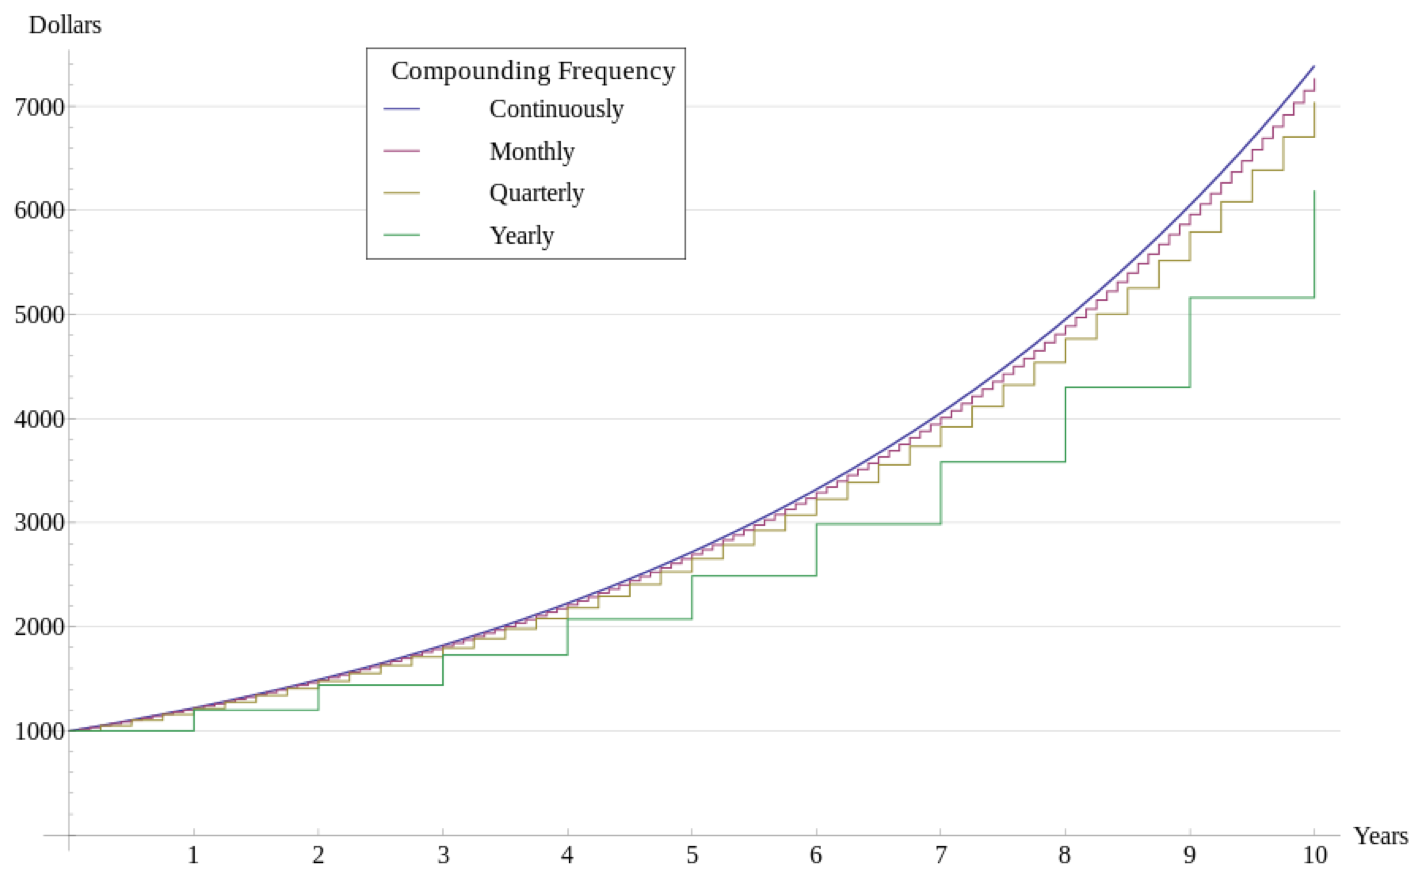
\includegraphics[width=0.9\linewidth]{money/interest.png}
\caption{年利率20\%的复利增长曲线}
\centering
\end{figure}

上面的故事实际上是一个虚构的故事,雅克比·伯努利(1654-1705)历史上实际上是一个
非常有名的数学家,他家虽然非常有钱,但他不是财主,也不放贷。但是他在生活中观察
到了放贷和利息计算这种行为,并对此进行了细致的研究,最终给出了复利的终极计算方
式,这个终极的计算方式里就包含了$e$。

\begin{figure}[htbp]
\centering
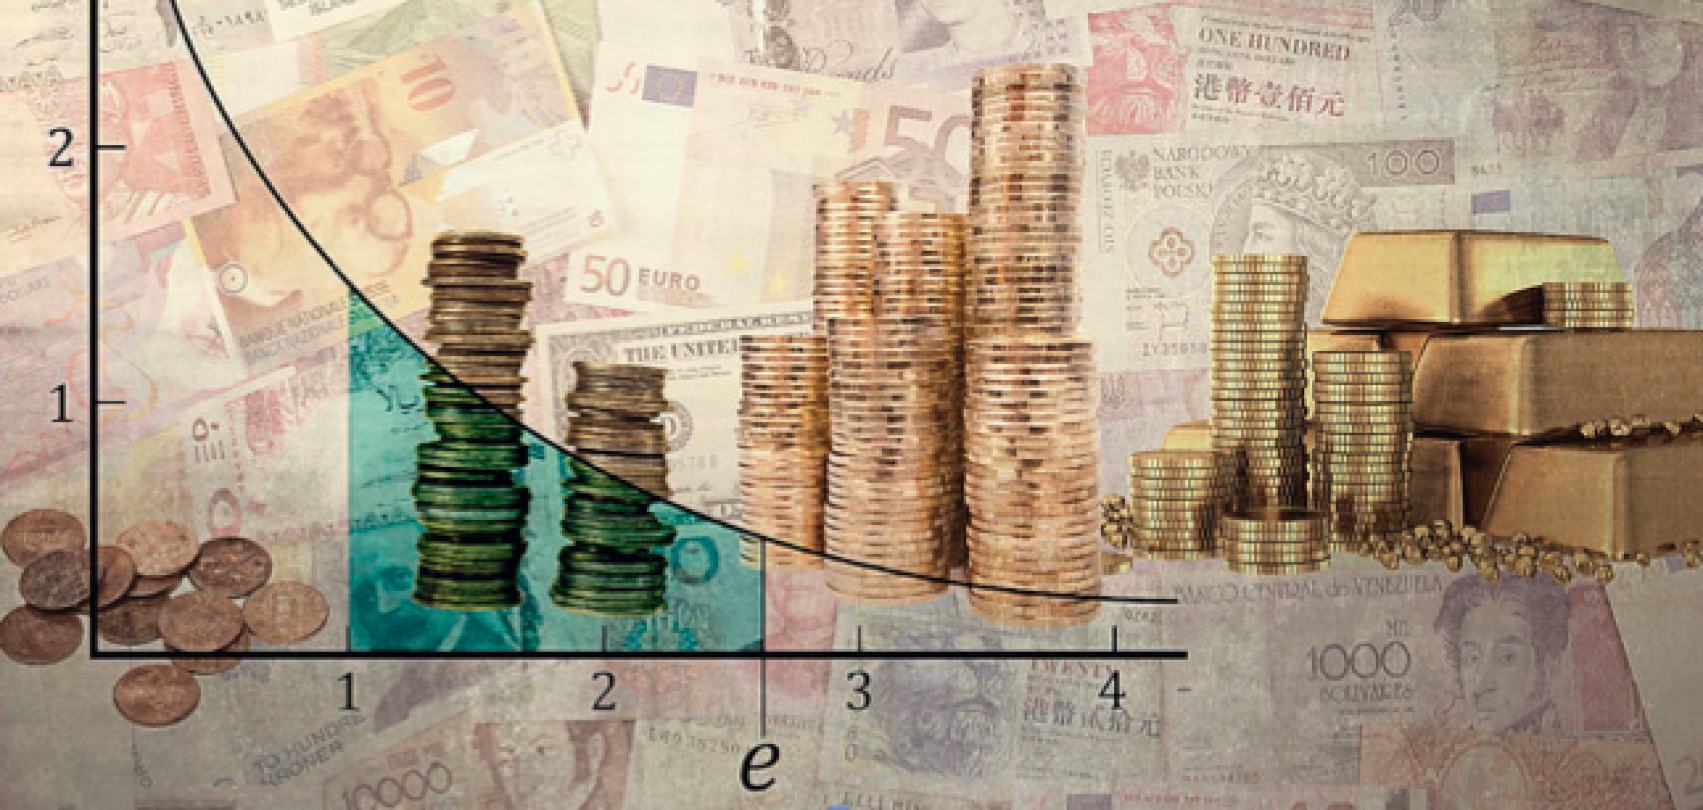
\includegraphics[width=0.9\linewidth]{money/e-interest.png}
\caption{$ e$ 与利息}
\centering
\end{figure}

在在瑞士苏黎世召开的1994年第22届国际数学家大会上,瑞士邮政发行的纪念邮票的邮票
图案就是雅各布·伯努利的头像,和以他名字命名的大数定律及大数定律的几何示意图。最
后告诫大家千万别找数学家借钱,数学家会把每一分该得的钱都计算的清清楚楚,分毫不
差。

\begin{figure}[htbp]
\centering
\begin{minipage}[t]{.45\linewidth}
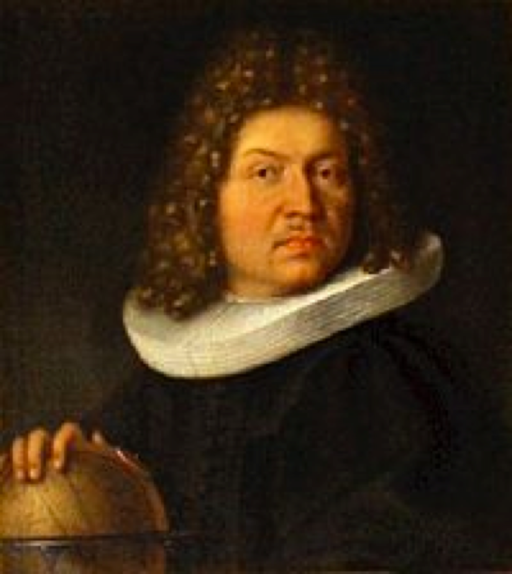
\includegraphics[height=1.8in]{money/bernoulli.png}
\caption{Jakob Bernoulli}
\end{minipage}
\begin{minipage}[t]{.45\linewidth}
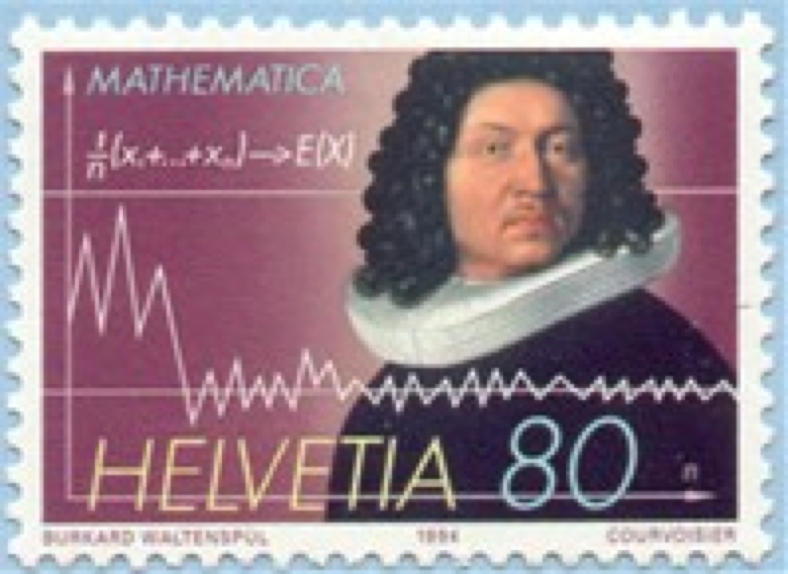
\includegraphics[width=\textwidth]{money/stamp.png}
\caption{纪念邮票}
\end{minipage}
\end{figure}
